\documentclass[12pt,a4paper,oneside]{report}
\usepackage[utf8]{inputenc}
\usepackage[english,russian]{babel}
\usepackage{amsmath}
\usepackage{amssymb}
\usepackage{geometry}
\usepackage{sverb}
\usepackage{graphicx}
\usepackage{pdfpages}
\usepackage{url}
\usepackage{titlesec, blindtext, color}
\usepackage{listings}
\usepackage{pgfplots}
\pgfplotsset{compat=newest}
\graphicspath{{../}}
\DeclareGraphicsExtensions{.pdf,.png,.jpg}
\usepackage{tabularx}
\usepackage{subcaption}
\usepackage{colortbl}
\usepackage{multirow}
\usepackage{longtable}
\usepackage{enumitem}
\usepackage{algorithm}
\usepackage{tikz}
\usepackage[noend]{algpseudocode}
\usepackage{float}
\usepackage{siunitx}


\definecolor{gray75}{gray}{0.75}
\definecolor{Blue}{HTML}{5D8AA8}
\newcommand{\hsp}{\hspace{20pt}}

\newcommand{\RomanNumeralCaps}[1]
{\MakeUppercase{\romannumeral #1}}


% Для листинга кода:
\lstset{ %
	language=c,                 % выбор языка для подсветки (здесь это С)
	basicstyle=\small\sffamily, % размер и начертание шрифта для подсветки кода             % где поставить нумерацию строк (слева\справа)
	numberstyle=\tiny,           % размер шрифта для номеров строк
	stepnumber=1, 
	keywordstyle=\color{blue},% размер шага между двумя номерами строк
	numbersep=5pt,                % как далеко отстоят номера строк от подсвечиваемого кода
	showspaces=false,            % показывать или нет пробелы специальными отступами
	showstringspaces=false,      % показывать или нет пробелы в строках
	showtabs=false,             % показывать или нет табуляцию в строках
	frame=single,              % рисовать рамку вокруг кода
	tabsize=2,                 % размер табуляции по умолчанию равен 2 пробелам
	captionpos=t,              % позиция заголовка вверху [t] или внизу [b] 
	breaklines=true,           % автоматически переносить строки (да\нет)
	breakatwhitespace=false, % переносить строки только если есть пробел
	escapeinside={\#*}{*)}  % Стиль литералов
}


\titleformat{\chapter}[hang]{\Huge\bfseries}{\thechapter.\textcolor{gray75}\hsp}{0pt}{\Huge\bfseries}
\newcommand{\specchapter}[1]{\chapter*{#1}\addcontentsline{toc}{chapter}{#1}}
\newcommand{\specsection}[1]{\section*{#1}\addcontentsline{toc}{section}{#1}}
\newcommand{\specsubsection}[1]{\subsection*{#1}\addcontentsline{toc}{subsection}{#1}}

% геометрия


\setcounter{tocdepth}{4} % фикс переноса 
\righthyphenmin = 2
\tolerance = 2048


\thispagestyle{empty}

\geometry{pdftex, left = 3cm, right = 1cm, top = 2cm, bottom = 2cm}


\begin{document}


% геометрия


\setcounter{tocdepth}{4} % фикс переноса 
\righthyphenmin = 2
\tolerance = 2048


\thispagestyle{empty}

\thispagestyle{empty}
\noindent \begin{minipage}{0.15\textwidth}
	
\includegraphics[width=\linewidth]{b_logo}
\end{minipage}
\noindent\begin{minipage}{0.9\textwidth}\centering
	\textbf{Министерство науки и высшего образования Российской Федерации}\\
	\textbf{Федеральное государственное бюджетное образовательное учреждение высшего образования}\\
	\textbf{«Московский государственный технический университет имени Н.Э.~Баумана}\\
	\textbf{(национальный исследовательский университет)»}\\
	\textbf{(МГТУ им. Н.Э.~Баумана)}
\end{minipage}
\noindent\rule{18cm}{3pt}
\newline\newline
\noindent ФАКУЛЬТЕТ $\underline{\textbf{«ИНФОРМАТИКА И СИСТЕМЫ УПРАВЛЕНИЯ»}}$ \newline\newline
\noindent КАФЕДРА $\underline{\textbf{«ПРОГРАММНОЕ ОБЕСПЕЧЕНИЕ ЭВМ И ИНФОРМАЦИОННЫЕ}}$\newline\newline $\underline{\textbf{ТЕХНОЛОГИИ»(ИУ7)}}$\newline\newline
\noindent НАПРАВЛЕНИЕ ПОДГОТОВКИ $\underline{\textbf{09.03.04 ПРОГРАММНАЯ ИНЖЕНЕРИЯ}}$\newline\newline\newline\newline\newline\newline\newline
\begin{center}
    \begin{flushright}
    \Large\textbf{ОТЧЕТ}\newline
	\Large\textbf{по лабораторной работе № 5}\newline
	\end{flushright}
\end{center}
\noindent\textbf{Название:} $\underline{\text{Определение вероятности отказа}}$\newline\newline
\noindent\textbf{Дисциплина:} $\underline{\text{Моделирование}}$\newline\newline\newline\newline\newline\newline\newline\newline
\begin{tabular}{lcp{5em}lp{2em}l}
	\noindent\textbf{Студент} &  $\underline{\text{ИУ7-71Б~~}}$ &             &\hspace{1cm} & & $\underline{\text{В.С.Плотников}}$ \\\cline{4-3}
	 & (Группа) & &(Подпись,дата)  & & (И.О.Фамилия) \\
	 & & & & &\\
	\noindent\textbf{Преподаватель} &  & &\hspace{1cm} & &$\underline{\text{И.В.Рудаков ~~~~}}$ \\\cline{4-3} 
	 &  & & (Подпись,дата)  & &(И.О.Фамилия) \\
    \end{tabular}
\begin{center}
	\vfill
	Москва, \the\year
\end{center}
\clearpage



\section*{Задание лабораторной работы}
\quad В информационный центр приходят клиенты через интервал времени $\SI{10}{} \pm \SI{2}{}$ минуты. Если все три имеющихся оператора заняты, клиенту отказывают в обслуживании. Операторы имеют разную производительность и могут обеспечивать обслуживание среднего запроса пользователя за $\SI{20}{} \pm \SI{5}{}$; $\SI{40}{} \pm \SI{10}{}$; $\SI{40}{} \pm \SI{20}{}$. Клиенты стремятся занять свободного оператора с максимальной производительностью. Полученные запросы сдаются в накопитель. Откуда выбираются на обработку. На первый компьютер запросы от 1 и 2-ого операторов, на второй – запросы от 3-его. Время обработки запросов первым и 2-м компьютером равны соответственно 15 и 30 мин. Промоделировать процесс обработки 300 запросов. 


\section*{Теоретическая часть}
\quad Для выполнения поставленного задания необходимо создать концептуальную модель в терминах СМО, определить эндогенные и экзогенные переменные и уравнения модели. За единицу системного времени выбрать 0,01 минуты.

\section*{}
\begin{figure}[!h]
	\centering
	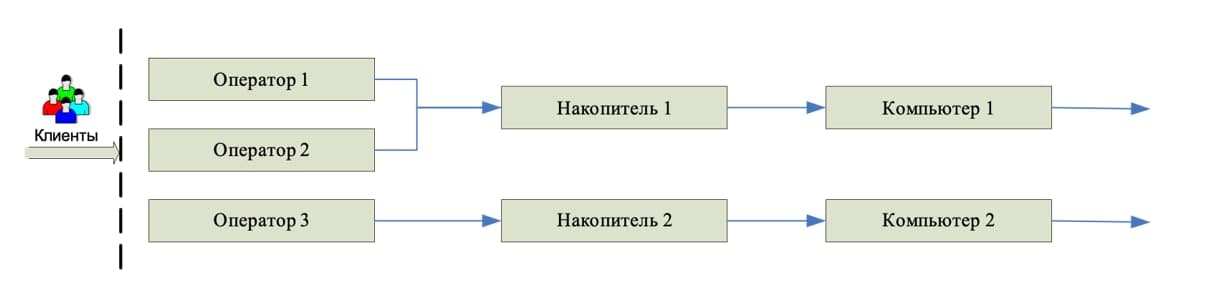
\includegraphics[scale=0.5]{teor_1.jpg}
	\label{fig:screenshot001}
\end{figure}

\quad В процессе взаимодействия клиентов с информационным центром возможно:

\begin{enumerate} 
  \item Режим нормального обслуживания, т.е. клиент выбирает одного из свободных операторов, отдавая предпочтение тому у которого меньше номер.
  \item Режим отказа в обслуживании клиента, когда все операторы заняты. 
\end{enumerate}

\quad Переменные и уравнения имитационной модели 
\begin{enumerate} 
  \item Эндогенные переменные: время обработки задания i-ым оператором, время решения этого задания j-ым компьютером.
  \item Экзогенные переменные: число обслуженных клиентов и число клиентов, получивших отказ.
\end{enumerate}

\newpage
\section*{}
\begin{figure}[!h]
	\centering
	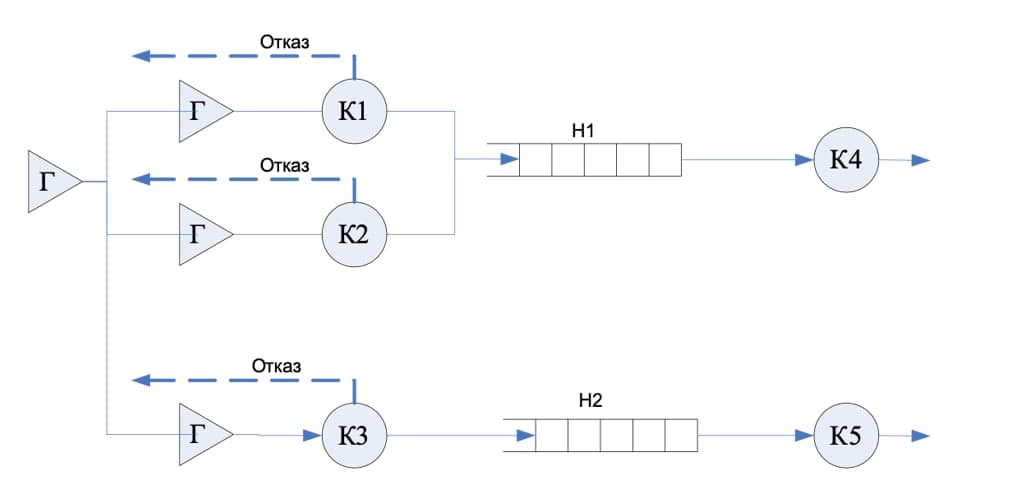
\includegraphics[scale=0.5]{teor_2.jpg}
	\label{fig:screenshot002}
\end{figure}

\begin{equation}
    P_{\text{отк}} = \frac{C_{\text{отк}}}{C_{\text{отк}} + C_{\text{обсл}}}  
\end{equation}


\newpage
\section*{Результат работы}
\begin{figure}[!h]
	\centering
	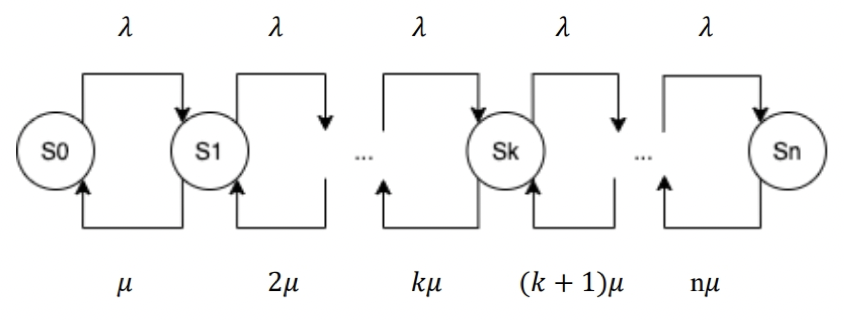
\includegraphics[scale=0.7]{1.png}
	\label{fig:screenshot003}
\end{figure}

\begin{figure}[!h]
	\centering
	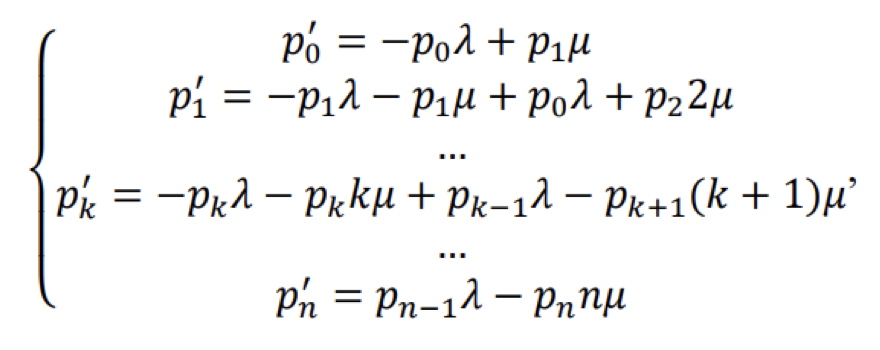
\includegraphics[scale=0.7]{2.png}
	\label{fig:screenshot004}
\end{figure}

\begin{figure}[!h]
	\centering
	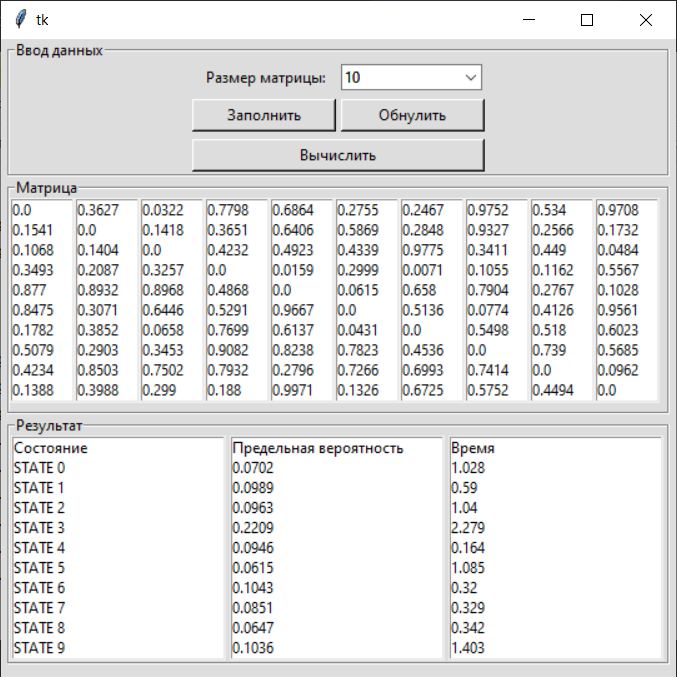
\includegraphics[scale=0.7]{3.png}
	\label{fig:screenshot005}
\end{figure}

\begin{figure}[!h]
	\centering
	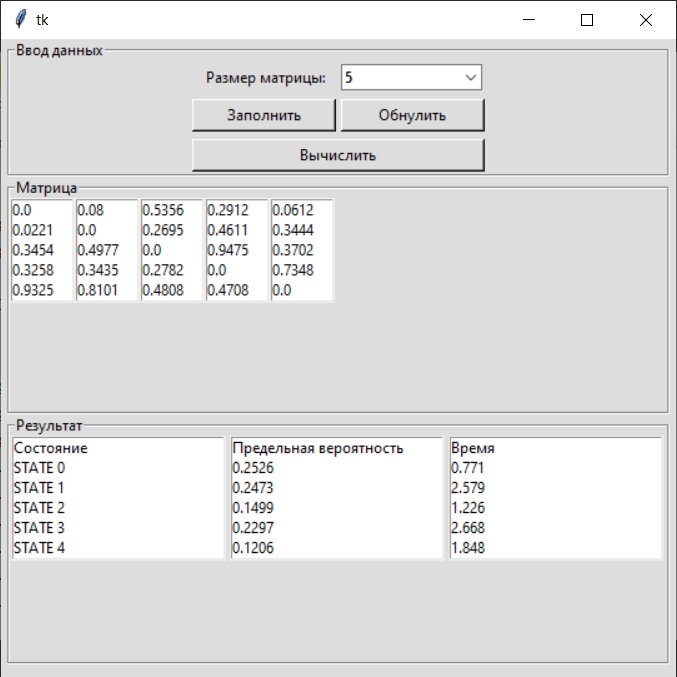
\includegraphics[scale=0.7]{4.png}
	\label{fig:screenshot006}
\end{figure}

\begin{figure}[!h]
	\centering
	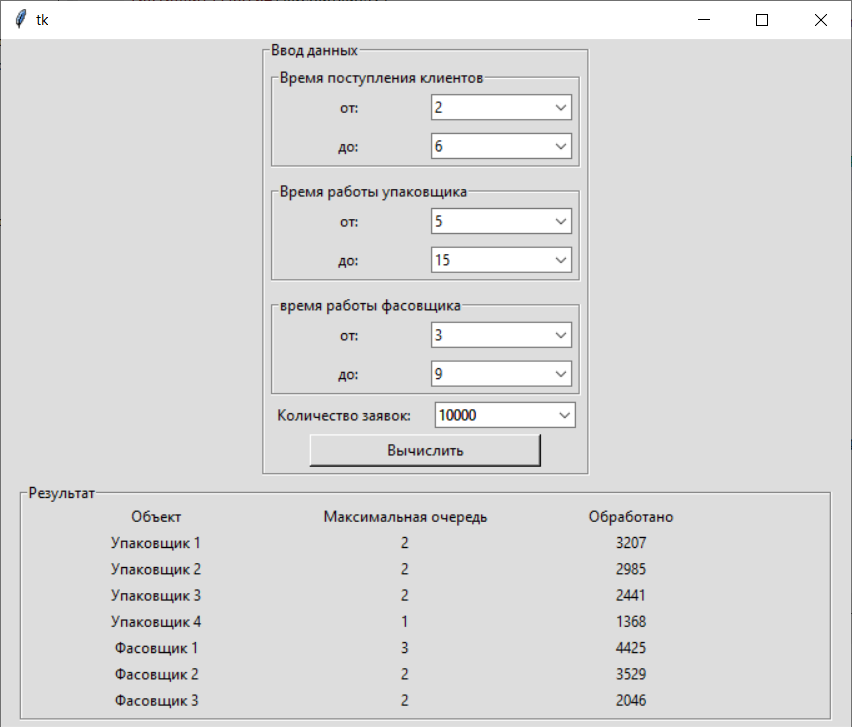
\includegraphics[scale=0.7]{5.png}
	\label{fig:screenshot007}
\end{figure}

\clearpage
\newpage

\section*{Вывод}
При следующих настройках информационного центра:

\begin{figure}[!h]
	\centering
	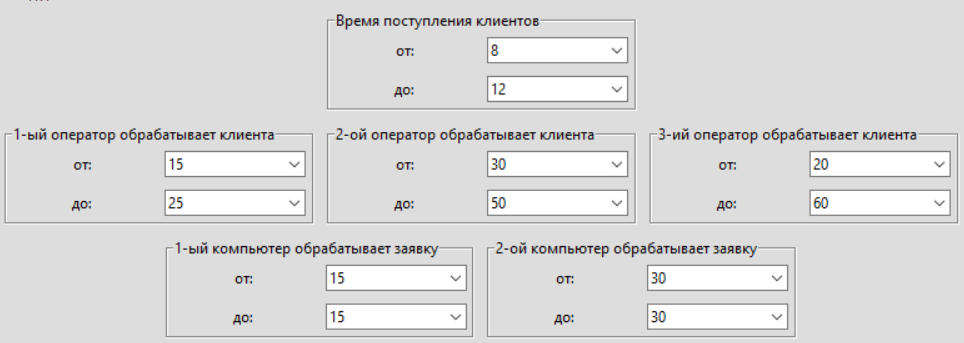
\includegraphics[scale=0.8]{sett.png}
	\label{fig:screenshot008}
\end{figure}

получены результаты:

\begin{table}[h]
	\centering
	\label{tbl:auth_user}
	\begin{tabular}{|l|l|l|l|}
		\hline
		\textbf{} & \textbf{\% потерь}  \\ \hline
		 100 клиентов & 23.00 \\ \hline
		 300 клиентов & 22.67 \\ \hline
		 1000 клиентов & 21.80 \\ \hline
	     3000 клиентов & 21.00 \\ \hline
	     10000 клиентов & 21.47 \\ \hline
	\end{tabular}
\end{table}

Таким образом, можно сделать вывод об объеме потерянных клиентов. При 300 клиентах получен результат 22.67 \%. Примерно такой же результат был получен и для других значений общего числа клиентов. 
\end{document}

